\documentclass[a4paper,12pt]{article} 
\usepackage[T2A]{fontenc}			
\usepackage[utf8]{inputenc}			
\usepackage[english,russian]{babel}	
\usepackage{amsmath,amsfonts,amssymb,amsthm,mathrsfs,mathtools} 
\usepackage{cancel}
\usepackage{multirow}
\usepackage[colorlinks, linkcolor = blue]{hyperref}
\usepackage{upgreek}\usepackage[left=2cm,right=2cm,top=2cm,bottom=3cm,bindingoffset=0cm]{geometry}
\usepackage{graphicx,wrapfig,subfig}
\usepackage{xcolor}
\author{Дорогинин Д.В.\\
Группа Б02-825}
\title{3.2.4. Свободные колебания в электрическом контуре.}
\date{}
\begin{document}
\maketitle
\textbf{Цель работы}: исследования свободных колебаний в колебательном контуре.


\textbf{В работе используются}: генератор импульсов, электронное реле, магазин сопротивлений, магазин ёмкостей, индуктивность, электронный осциллограф, унивенрсальный мост.
\section*{Теория}
\subsection*{Свободные колебания}
\begin{wrapfigure}{r}{5cm}
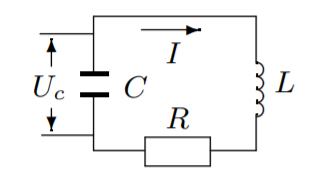
\includegraphics[scale=0.7]{2.png}
\end{wrapfigure}
Рассмотрим электрический контур, состоящий из последовательно соединённых конденстора $C$, катушки индуктивности $L$ и резистора $R$. Обозначим разность потенциалов на конденсаторе $U_C$, а ток, текущий в контуре, через $I$. Второе првило Кирхгофа:
\begin{equation}
L \dfrac{d^2I}{dt^2}+R\dfrac{dI}{dt}+\dfrac{I}{C}=0.
\end{equation}
Вводя обозначения $\gamma = \dfrac{R}{2L}$, $\omega_0^2=\dfrac{1}{LC}$, получим уравнение
\begin{equation}
\ddot{I}+2\gamma\dot{I}+\omega_0^2I=0.
\end{equation}
Его решение в общем виде:
\begin{equation}
I = -\dfrac{U_0}{L\kappa}e^{-\gamma t}\text{sh}(\kappa t), 
\end{equation}
где $\kappa = \sqrt{\gamma^2 - \omega_0^2}$, $U_0 = U_C$ -- начальное напряжение на конденсаторе.

\subsection*{Затухающие колебания}
\begin{wrapfigure}{r}{8cm}
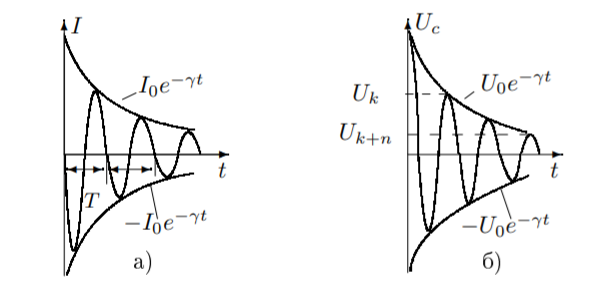
\includegraphics[scale=0.6]{3.png}
\caption{Затухающие колебания.}
\vspace{-30pt}
\end{wrapfigure}
 В случае, когда $\gamma < \omega_0$, имеем $\kappa = i\omega$, где $\omega = \sqrt{\omega_0^2 - \gamma^2}$ -- \textit{частоты свободных (собственных) колебаний}. Тогда ток
 \begin{equation}
 I = -\dfrac{U_0}{L\omega}e^{-\gamma t}\sin(\omega t)
 \end{equation}
 затухает и имеет колебательный характер. Величина $\gamma$ определяет затухание колебаний: $\gamma = \dfrac{1}{\tau}$, где $\tau$ -- время затухание амплитуды в $e$ раз.
Формулы для наряжение на кондесаторе и тока в цепи можно переписать иначе:
\begin{equation}
\begin{array}{c}
U_C = U_0 \dfrac{\omega_0}{\omega}e^{-\gamma t} \cos(\omega t - \theta),\\
\\
I = -\dfrac{U_0}{L}e^{-\gamma t} \cos(\omega t - \theta).
\end{array}
\end{equation}
\subsection*{Апериодические колебания}
В случае $\gamma > \omega_0$, формулы для тока и напряжения на конденсаторе имеют следующий вид:

\begin{wrapfigure}{r}{8.5cm}
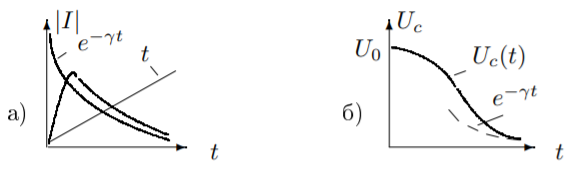
\includegraphics[scale=0.7]{4.png}
\caption{Критический режим.}
\vspace{-40pt}
\end{wrapfigure}
$$
\begin{array}{c}
I = -\dfrac{U_0}{L\kappa}e^{-\gamma t}\text{sh}(\kappa t),\\
\\
U_C = U_0 e^{-\gamma t}\left( \dfrac{\gamma}{\kappa}\text{sh}(\kappa t) + \text{ch}(\kappa t) \right).
\end{array}
$$
Процесс в этом случае не является колебательным, его называют апериодическим. Режим, соответствующий $\gamma = \omega_0$, называются \textit{критическим}. В этом случае предельный переход $\omega \rightarrow 0$ в $(5)$ даст 
$$
\begin{array}{c}
I = -\dfrac{U_0}{L}te^{-\gamma t},\\
\\
U_C=U_0 e^{-\gamma t}(1+\gamma t).
\end{array}
$$
Сопротивление в этом случае 
\begin{equation}
R_{\text{кр}}= 2 \sqrt{\dfrac{L}{C}}
\end{equation}
называется \textit{критическим сопротивлением} контура.\\
\textit{Добротность} контура по определению 
$$
Q = 2\pi \dfrac{W}{\Delta W},
$$ 
где $W$ -- запасённая энергия, $\Delta W$ -- потери за период. Тогда
\begin{equation}
Q = 2\pi\dfrac{CU_0^2/2 \cdot e^{-2\gamma t}}{CU_0^2/2 \cdot (e^{-2\gamma t} - e^{-2\gamma (T+t)})}=\dfrac{\pi}{\gamma T}=\dfrac{1}{R}\sqrt{\dfrac{L}{C}}.
\end{equation}
\textit{Логарифмическим декрементом затухания} называются число
\begin{equation}
\Theta = \text{ln}\dfrac{U_k}{U_{k+1}}=\text{ln} e^{\gamma T}=\gamma T.
\end{equation}
или 
\begin{equation}
\Theta = \dfrac{1}{n} \text{ln}\dfrac{U_k}{U_{k+n}}.
\end{equation}
\section*{Описание установки}
\begin{center}
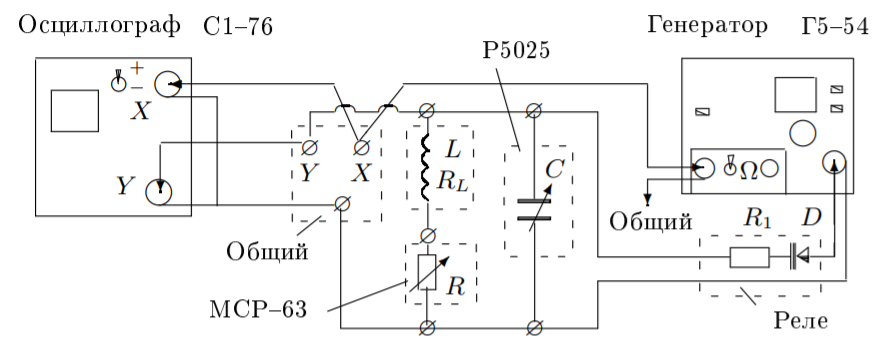
\includegraphics[scale=0.6]{1.png}
\end{center}
На рисунке приведена схема для исследования свободных колебаний в контуре, содержащем постоянную индуктивность $L$ и переменные ёмкость $C$ и сопротивление $R$. Колебания наблюдаются на экране осциллографа.\\
Для периодического возбуждения колебаний в контуре используется генератор импульсов Г5-54. С выхода генератора по коаксиальному кабелю импульсы поступают на колебательный контур через электронное реле, смонтированное в отдельном блоке (или на выходе генератора). Реле содержит тиристор $D$ и ограничительный резистор $R_1$.\\
Импульсы заряжают конденсатор $C$. После каждого импульса генератор отключается от колебательного контура, и в контуре возникают свободные затухающие колебания. Входное сопротивление осциллографа велико ($\approx 1$ МОм), так что его влиянием на контур можно пренебречь. Для получения устойчивой картины затухающих колебаний используется режим ждущей развёртки с синхронизацией внешними импульсами, поступающими с выхода <<синхроимпульсы>> генератора.
\section*{Ход работы}
На генераторе устанавливаем длительность импульсов 5 мск, частоту повторения $\nu_0 = 100$ Гц. На магазине сопротивлений устанавливаем величину $R = 0$ Ом, на магазине ёмкостей -- $C = 0.02$ мкФ. По картине на осциллографе проведём измерение зависимости периода свободных колебаний от ёмкости.
\begin{table}[h]
\centering
\begin{tabular}{|c|c|c|c|c|c|c|c|c|}
\hline
$C$, мкФ    & 0.02 & 0.03 & 0.04 & 0.05 & 0.06 & 0.07 & 0.08 & 0.09 \\ \hline
$T$, мкс    & 0.33 & 0.43 & 0.48 & 0.50 & 0.57 & 0.62 & 0.64 & 0.73  \\ \hline
\end{tabular}
\caption{Зависимость $T = T(C)$.}
\end{table}\\
Считая $L \approx 200$ мГн, рассчитаем $C$, при которой $\nu_0 = 1/2\pi \sqrt{LC} = 5$ кГц: $C \approx 5$ нФ. Критическое сопротивление в этом случае $R_{\text{кр}} \approx 12500$ Ом. Измерим зависимость $\Theta(R)$ декремента затухания от сопротивления в диапазоне $0.1R_{\text{кр}}\div 0.3R_{\text{кр}}$, пользуясь формулой (9):
\begin{table}[h]
\centering
\begin{tabular}{|c|c|c|c|c|c|c|c|c|}
\hline
$R$, Ом     & 1200 & 1300 & 1700 & 2100 & 2500 & 2900 & 3400 & 3700 \\ \hline
$\Theta$ & 0.7  & 0.8  & 1.0  & 1.3  & 1.5  & 1.7  & 2.1  & 2.2  \\ \hline
\end{tabular}
\caption{Зависимость $\Theta = \Theta(R)$.}
\end{table}
\newpage
Получив изображение колебаний на фазовой плоскости (в координатах $\left(U_C, \dfrac{dU_C}{dt}\right)$, убеждаемся, что декремент затухания вычисленный по тем же способом абсолютно совпадает с вычисленным в кооридинатах $\left( U_C, t\right)$.
С помощью универсального моста измеряем индуктивность $L$ и $R_L$ катушки для трёх значений частоты:
\begin{table}[h]
\centering
\begin{tabular}{|c|c|c|c|}
\hline
$\nu$, Гц  & 50    & 1000  & 5000  \\ \hline
$R_L$, Ом & 10.39 & 11.40 & 13.50 \\ \hline
$L$, мГн & 147.0 & 143.0 & 143.5 \\ \hline
\end{tabular}
\caption{Значения $R_L$ и $L$ катушки при разных частотах.}
\end{table}
\section*{Обработка результатов}
Рассчитаем теоретически периоды свободных колебаний и сравним с полученными экспериментально:
\begin{table}[h]
\centering
\begin{tabular}{|c|c|c|c|c|c|c|c|c|}
\hline
$T_{\text{эксп}}$, мкс & 0.33 & 0.43 & 0.48 & 0.50 & 0.57 & 0.62 & 0.64 & 0.73 \\ \hline
$T_{\text{теор}}$, мкс & 0.34 & 0.41 & 0.48 & 0.53 & 0.59 & 0.63 & 0.68 & 0.72 \\ \hline
\end{tabular}
\caption{Сравнение теоретических и экспериментальных периодов.}
\end{table}\\
Результат представим на графике:
\begin{center}
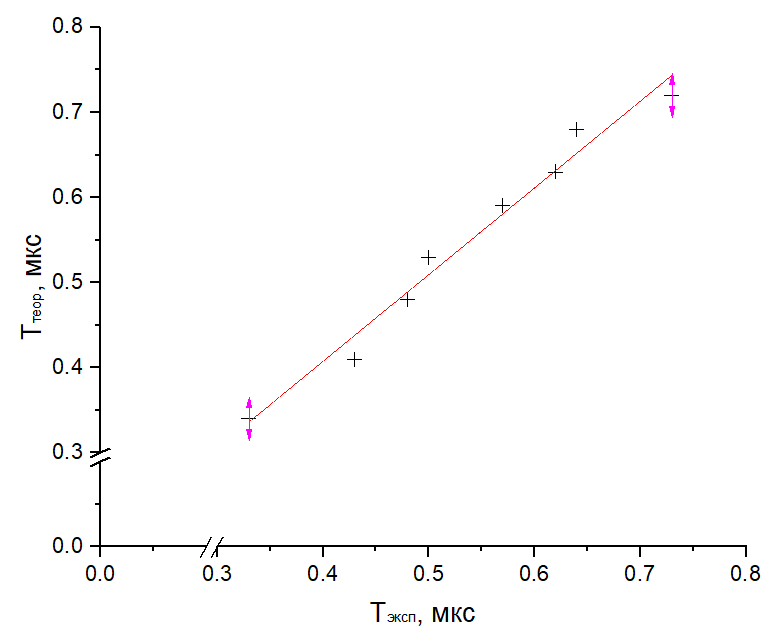
\includegraphics[scale=0.6]{5.png}
\end{center}
Для данных Таблицы 2 рассчитаем критическое сопротивление по формуле 
$$
R_{\text{кр}}=R\sqrt{\left( \dfrac{2\pi}{\Theta}\right)^2 + 1}
$$ 
и усредним:
\fbox{$R_{\text{кр}} = 10800 \pm 500~\text{Ом}$}\\
Теоретическое значение $R_{\text{кр}}=2\sqrt{\dfrac{L}{C}} = 10700 \pm 200$ Ом -- совпадает в пределах погрешности.\\
Для конутуров с максимальным и минимальным декрементом $\Theta$ рассчитаем добротность $Q$ экспериментальную -- $Q = \dfrac{\pi}{\Theta}$ -- и теоретическую -- $Q=\dfrac{1}{R}\sqrt{\dfrac{L}{C}}$:
\begin{table}[h]
\centering
\begin{tabular}{|c|c|c|c|c|}
\hline
     & $\Theta$      & $R$    & $Q_{\text{теор}}$         & $Q_{\text{эксп}}$  \\ \hline
Макс & $2.2 \pm 0.2$ & $3700$ & $1.443 \pm 0.012$ & $1.41 \pm 0.13$ \\ \hline
Мин  & $0.7 \pm 0.2$ & $1200$ & $4.45 \pm 0.04$   & $4.5 \pm 1.3  $ \\ \hline
\end{tabular}
\caption{Добротности для конутров с наибольшим и наименьшим затуханием.}
\end{table}
\end{document}